\documentclass{beamer}

\usetheme{Madrid}

\usepackage{graphicx}
\title{Stereo Sound System}

\subtitle{Independent Project}

\author{Sharad Roy - EE16B1029}


\institute[IIT Bhilai] 
{Department of Electrical Engineering \\
 Indian Institute of Technology Bhilai}


\date{28/04/2017}

\begin{document}

\begin{frame}
  \titlepage
\end{frame}

\section*{First Section}
\begin{frame}{Objective}
Our objective is to a make Stereo Sound System or simply an Audio Amplifier. We take the input signal from a device and then amplify it using the circuit and the output can be heard through speakers. 
\begin{block}{Components used:}

\begin{itemize}
    \item TEA2025 IC
    \item IC 7809 Voltage Regulator
    \item 9-V Step Down Transformer
    \item Potentiometer x 2
    \item Capacitors
    \item Speaker x 2
    
\end{itemize}
\end{block}
\end{frame}


\section*{Second Section}
\begin{frame}{IC 7809 Voltage Regulator}
 \begin{columns}
 \begin{column}{0.4\textwidth}
  \begin{block}{What is it?}
 IC 7809 is a 9V Voltage Regulator that restricts the voltage output to 9V and draws 9V regulated power supply. It regulates a steady output of 9V if the input voltage is in the range. \\
  There are 3 pins in IC 7809, pin 1 takes the input voltage and pin 3 produces the output voltage. The GND of both input and out are given to pin 2.
  \end{block}
  \end{column}
  
  \begin{column}{0.4\textwidth}
  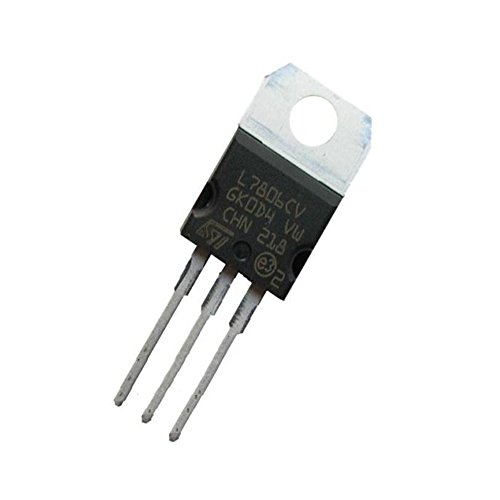
\includegraphics[width=\columnwidth]{IC.jpg}
  \end{column}
  
  \end{columns}
\end{frame}

\section*{Third Section}
\begin{frame}{TEA2025A IC}
\begin{columns}
\begin{column}{0.4\textwidth}
\begin{block}{About it}
The UTC TEA2025 is a monolithic integrated audio amplifier IC. It is capable of providing max. gain of 45dB. However, it can be lowered by placing an external RC series circuit between the feedback pin (6 and 11, see pin diagram) and ground. It has an inbuilt heat sink. The 0.1 $\mu F$ capacitors at the output end are for frequency stability. \end{block}
\end{column}

\begin{column}{0.4\textwidth}
\begin{block}{Circuit}

\includegraphics[width=\columnwidth]{text7088.png} \end{block}
\end{column}
\end{columns}
\end{frame}

\section*{Fourth Section}
\begin{frame}{Rectifying Circuit}
\centering
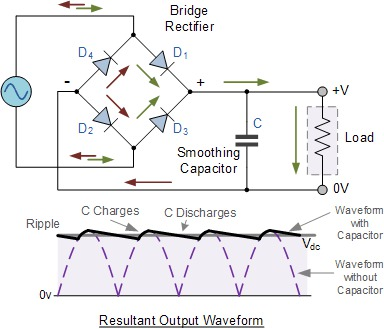
\includegraphics[scale=2]{diode23.jpg}
\end{frame}

\end{document}


